%%%%%%%%%%%%%%%%%%%%%%%%%%%%%%%%%%%%%%%%%%%%%%%%%%%%%%%%%%%%%%%%%%%%%%%%%%%%%%%%%%%%%%%%%%%%%%%%%%%%%%
%
%   Filename    : chapter_3.tex 
%
%   Description : This file will contain your Theoretical Framework.
%                 
%%%%%%%%%%%%%%%%%%%%%%%%%%%%%%%%%%%%%%%%%%%%%%%%%%%%%%%%%%%%%%%%%%%%%%%%%%%%%%%%%%%%%%%%%%%%%%%%%%%%%%

\chapter{Theoretical Framework}
\label{sec:theoframework}

\section{Convolutional Neural Networks}
Convolutional Neural Networks (CNNs) are the primary architecture for modern computer vision. They operate on grid‑structured data such as images. Learnable convolutional filters extract hierarchical visual features, progressing from simple edges to complex semantics. Given an input feature map $X$, a convolutional kernel $W$, and a bias term $b$, the resulting output feature map $Y$ is computed as
\begin{equation}
Y = W \ast X + b,
\end{equation}

\begin{figure}[h]
\centering
\caption{Illustration of IoU taken from the Aedes egg dataset.}
\label{fig:iou_explainer}
\end{figure}
where $\ast$ denotes the convolution operation. Each filter generates a corresponding output channel that encodes a specific learned visual representation, allowing the network to achieve translation invariance and parameter sharing.

\section{Object Detectors}
Building upon the feature extraction capabilities of CNNs, object detectors are specialized architectures tasked with simultaneously classifying objects within an image and localizing them through bounding box coordinates. This requires a multi-task learning approach where the model optimizes both a classification loss and a localization regression loss. Object detection architectures typically consist of distinct structural components responsible for feature extraction, multi-scale feature aggregation, and prediction, allowing for targeted architectural modifications.

\subsection{YOLO Architecture}

\begin{figure}[h]
\centering
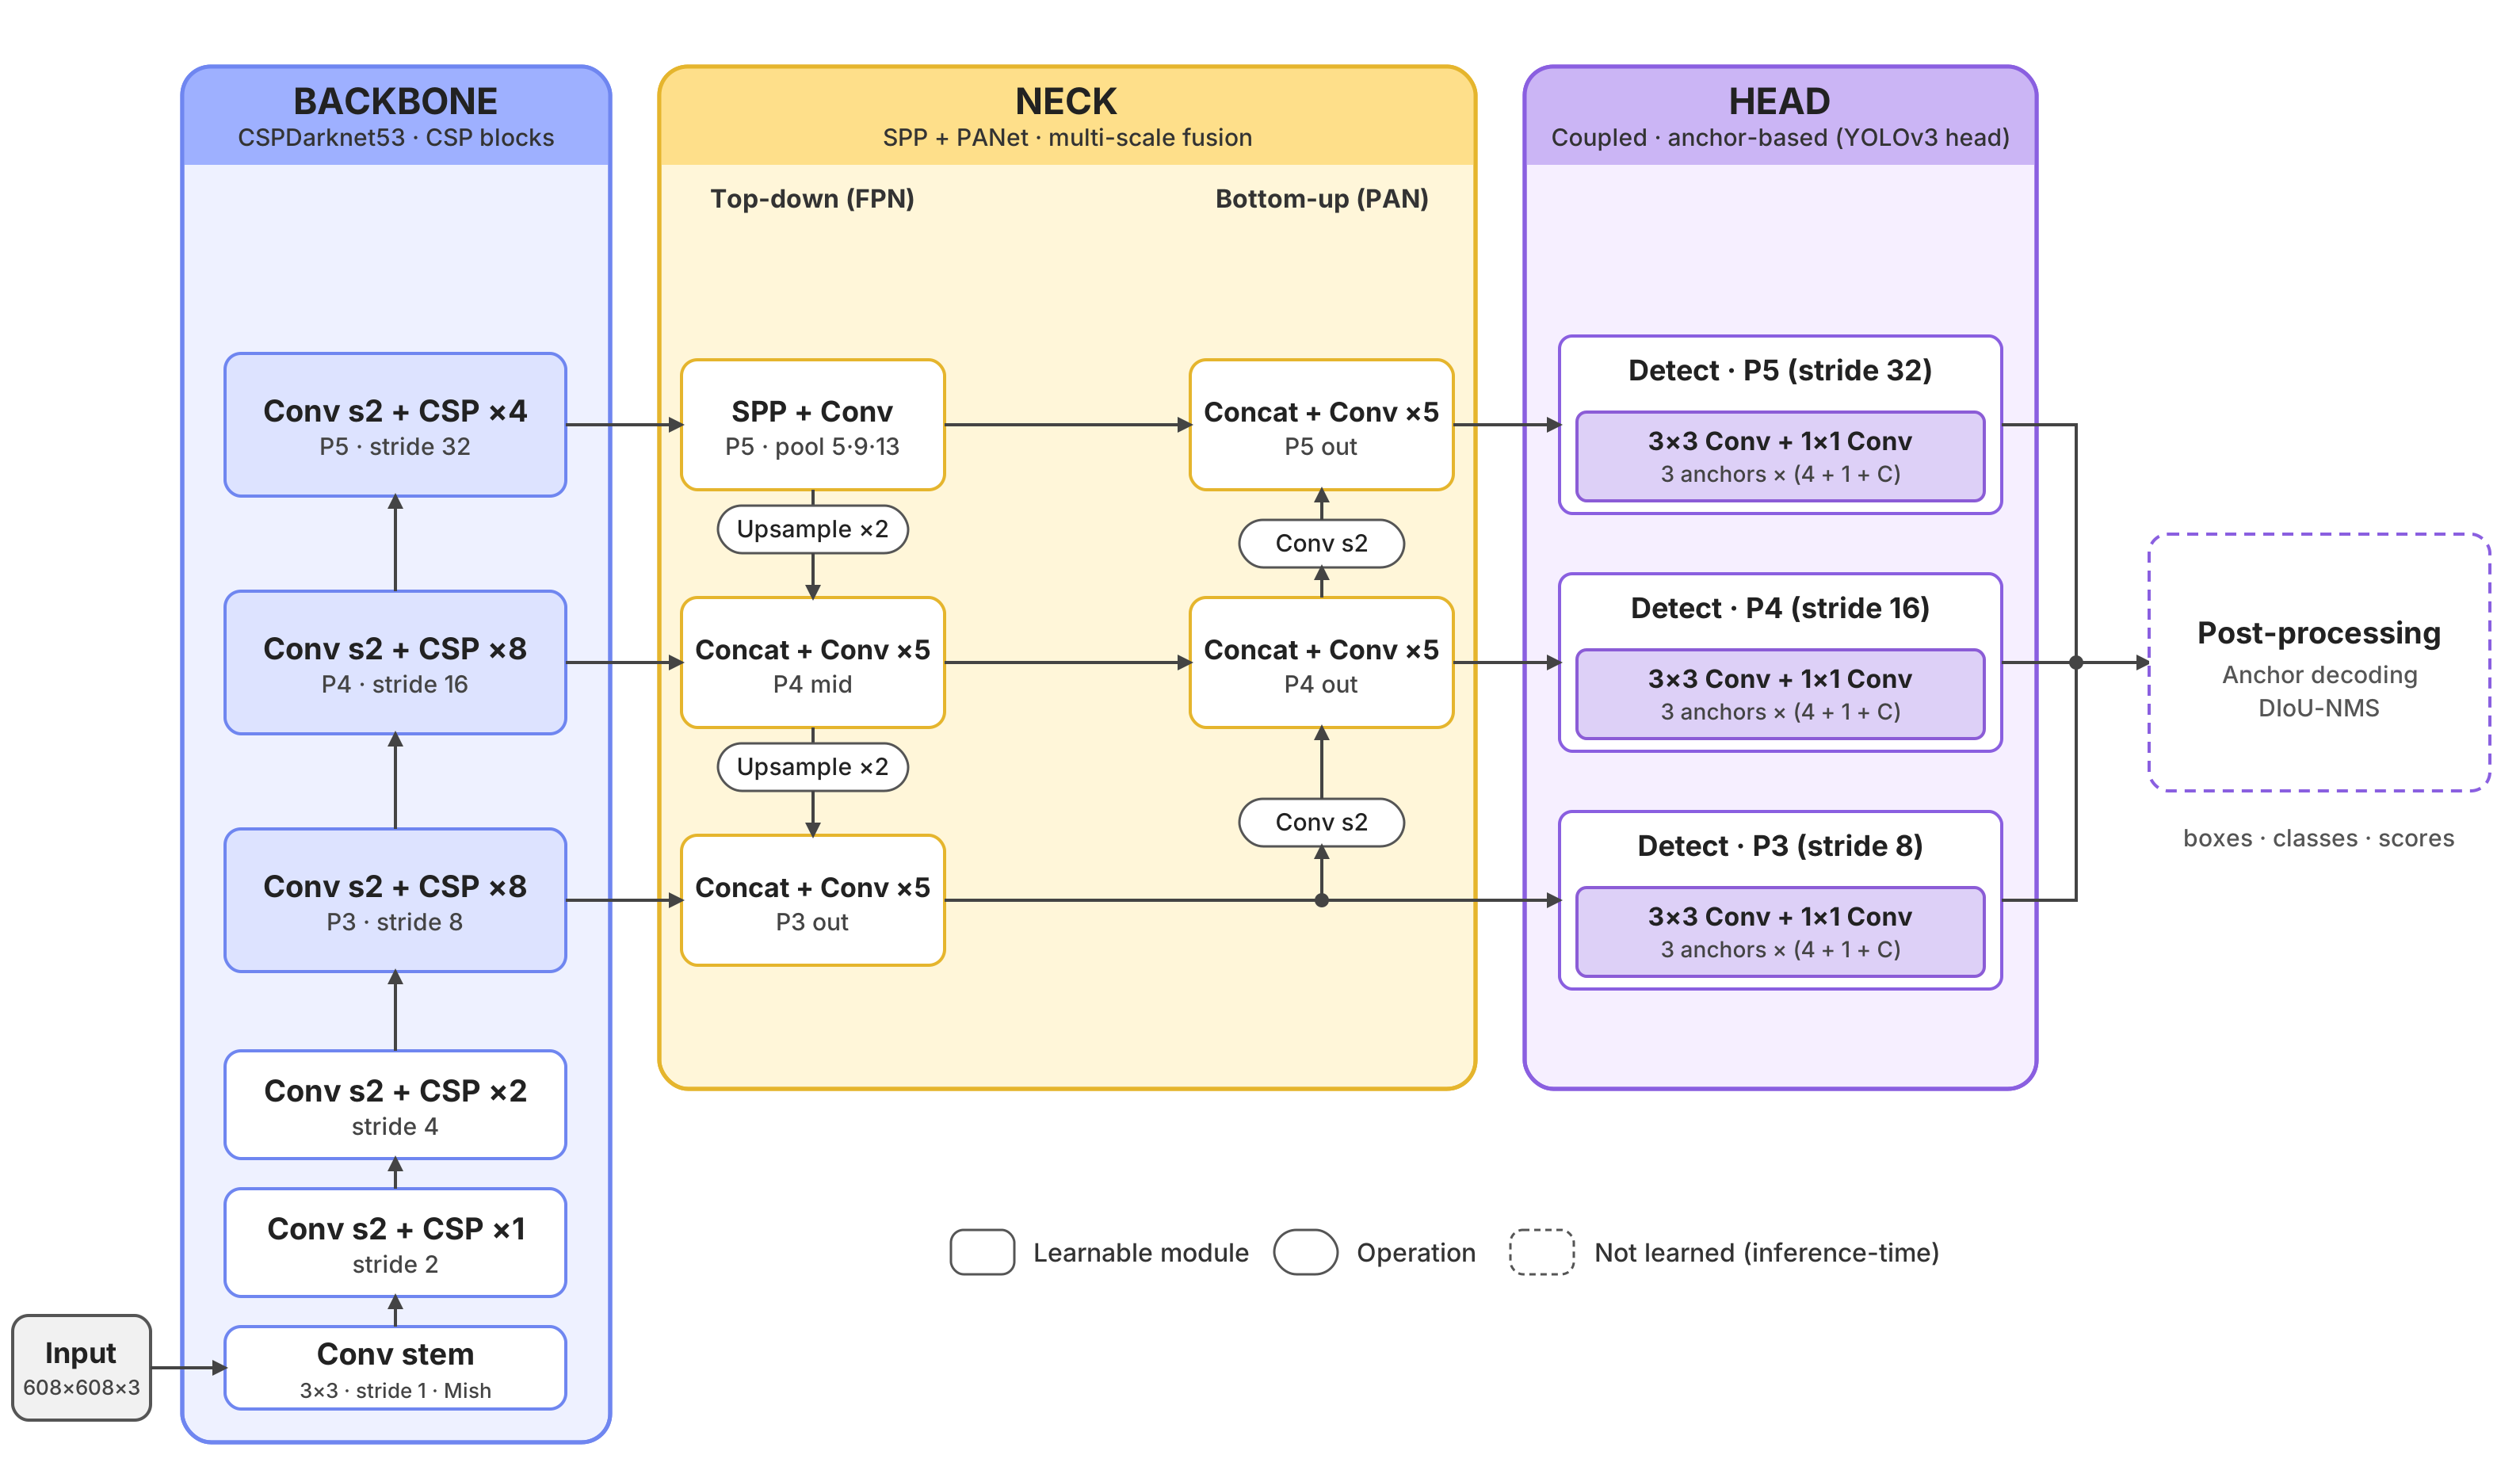
\includegraphics[width=\linewidth]{yolov4_architecture.png}
\caption{YOLOv4 architecture: backbone (CSPDarknet53), neck (SPP + PANet), and YOLOv3‑style head.}
\label{fig:yolov4_arch}
\end{figure}

\begin{figure}[h]
\centering
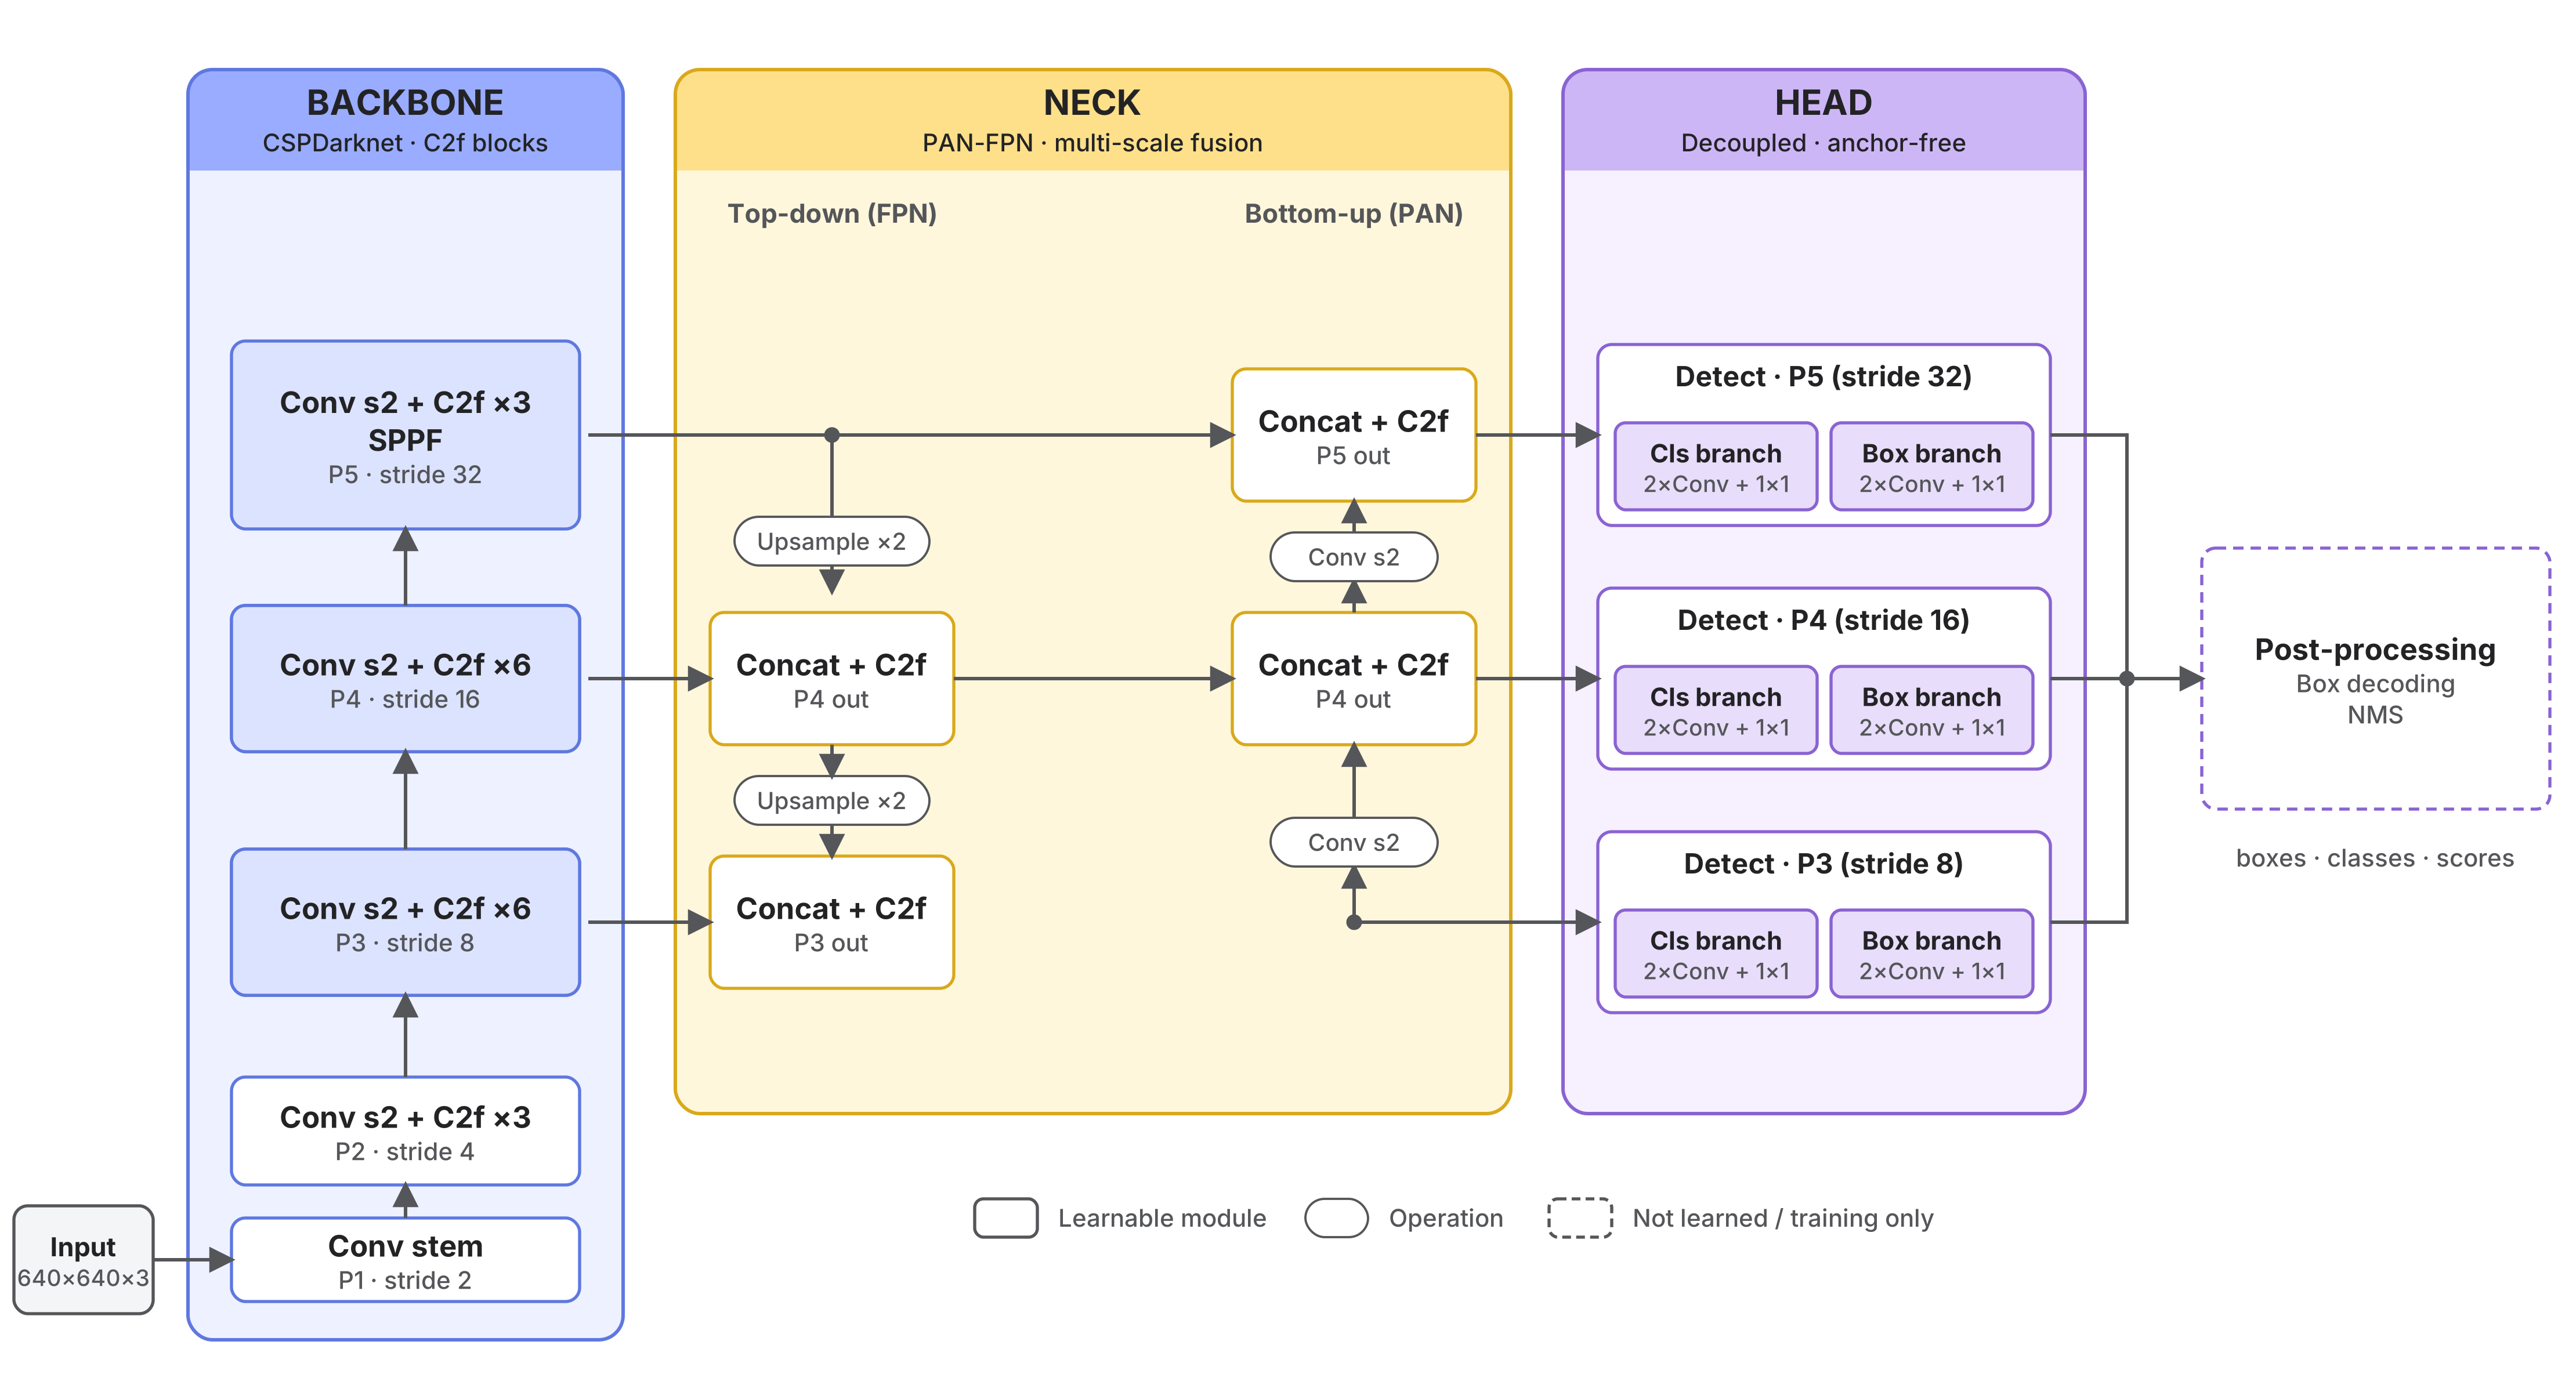
\includegraphics[width=\linewidth]{yolo_architecture (1).png}
\caption{YOLOv8 architecture: CSPDarknet backbone with C2f blocks, SPPF, and decoupled anchor‑free head.}
\label{fig:yolov8_arch}
\end{figure}
The You Only Look Once (YOLO) family of models represents the single-stage approach to object detection, framing the task as a single regression problem to achieve high inference speeds. Structurally, the architecture is divided into three primary components: the backbone, the neck, and the detection head. The backbone is responsible for extracting hierarchical features from the raw input image. The neck aggregates and fuses these features across multiple spatial scales to preserve contextual information for objects of varying sizes. Finally, the detection head performs dense predictions to output the final bounding box coordinates and class probabilities. This explicit modular separation makes each component a distinct candidate for structural pruning based on its inherent redundancy.

\subsection{DETR Architecture}

\begin{figure}[h]
\centering
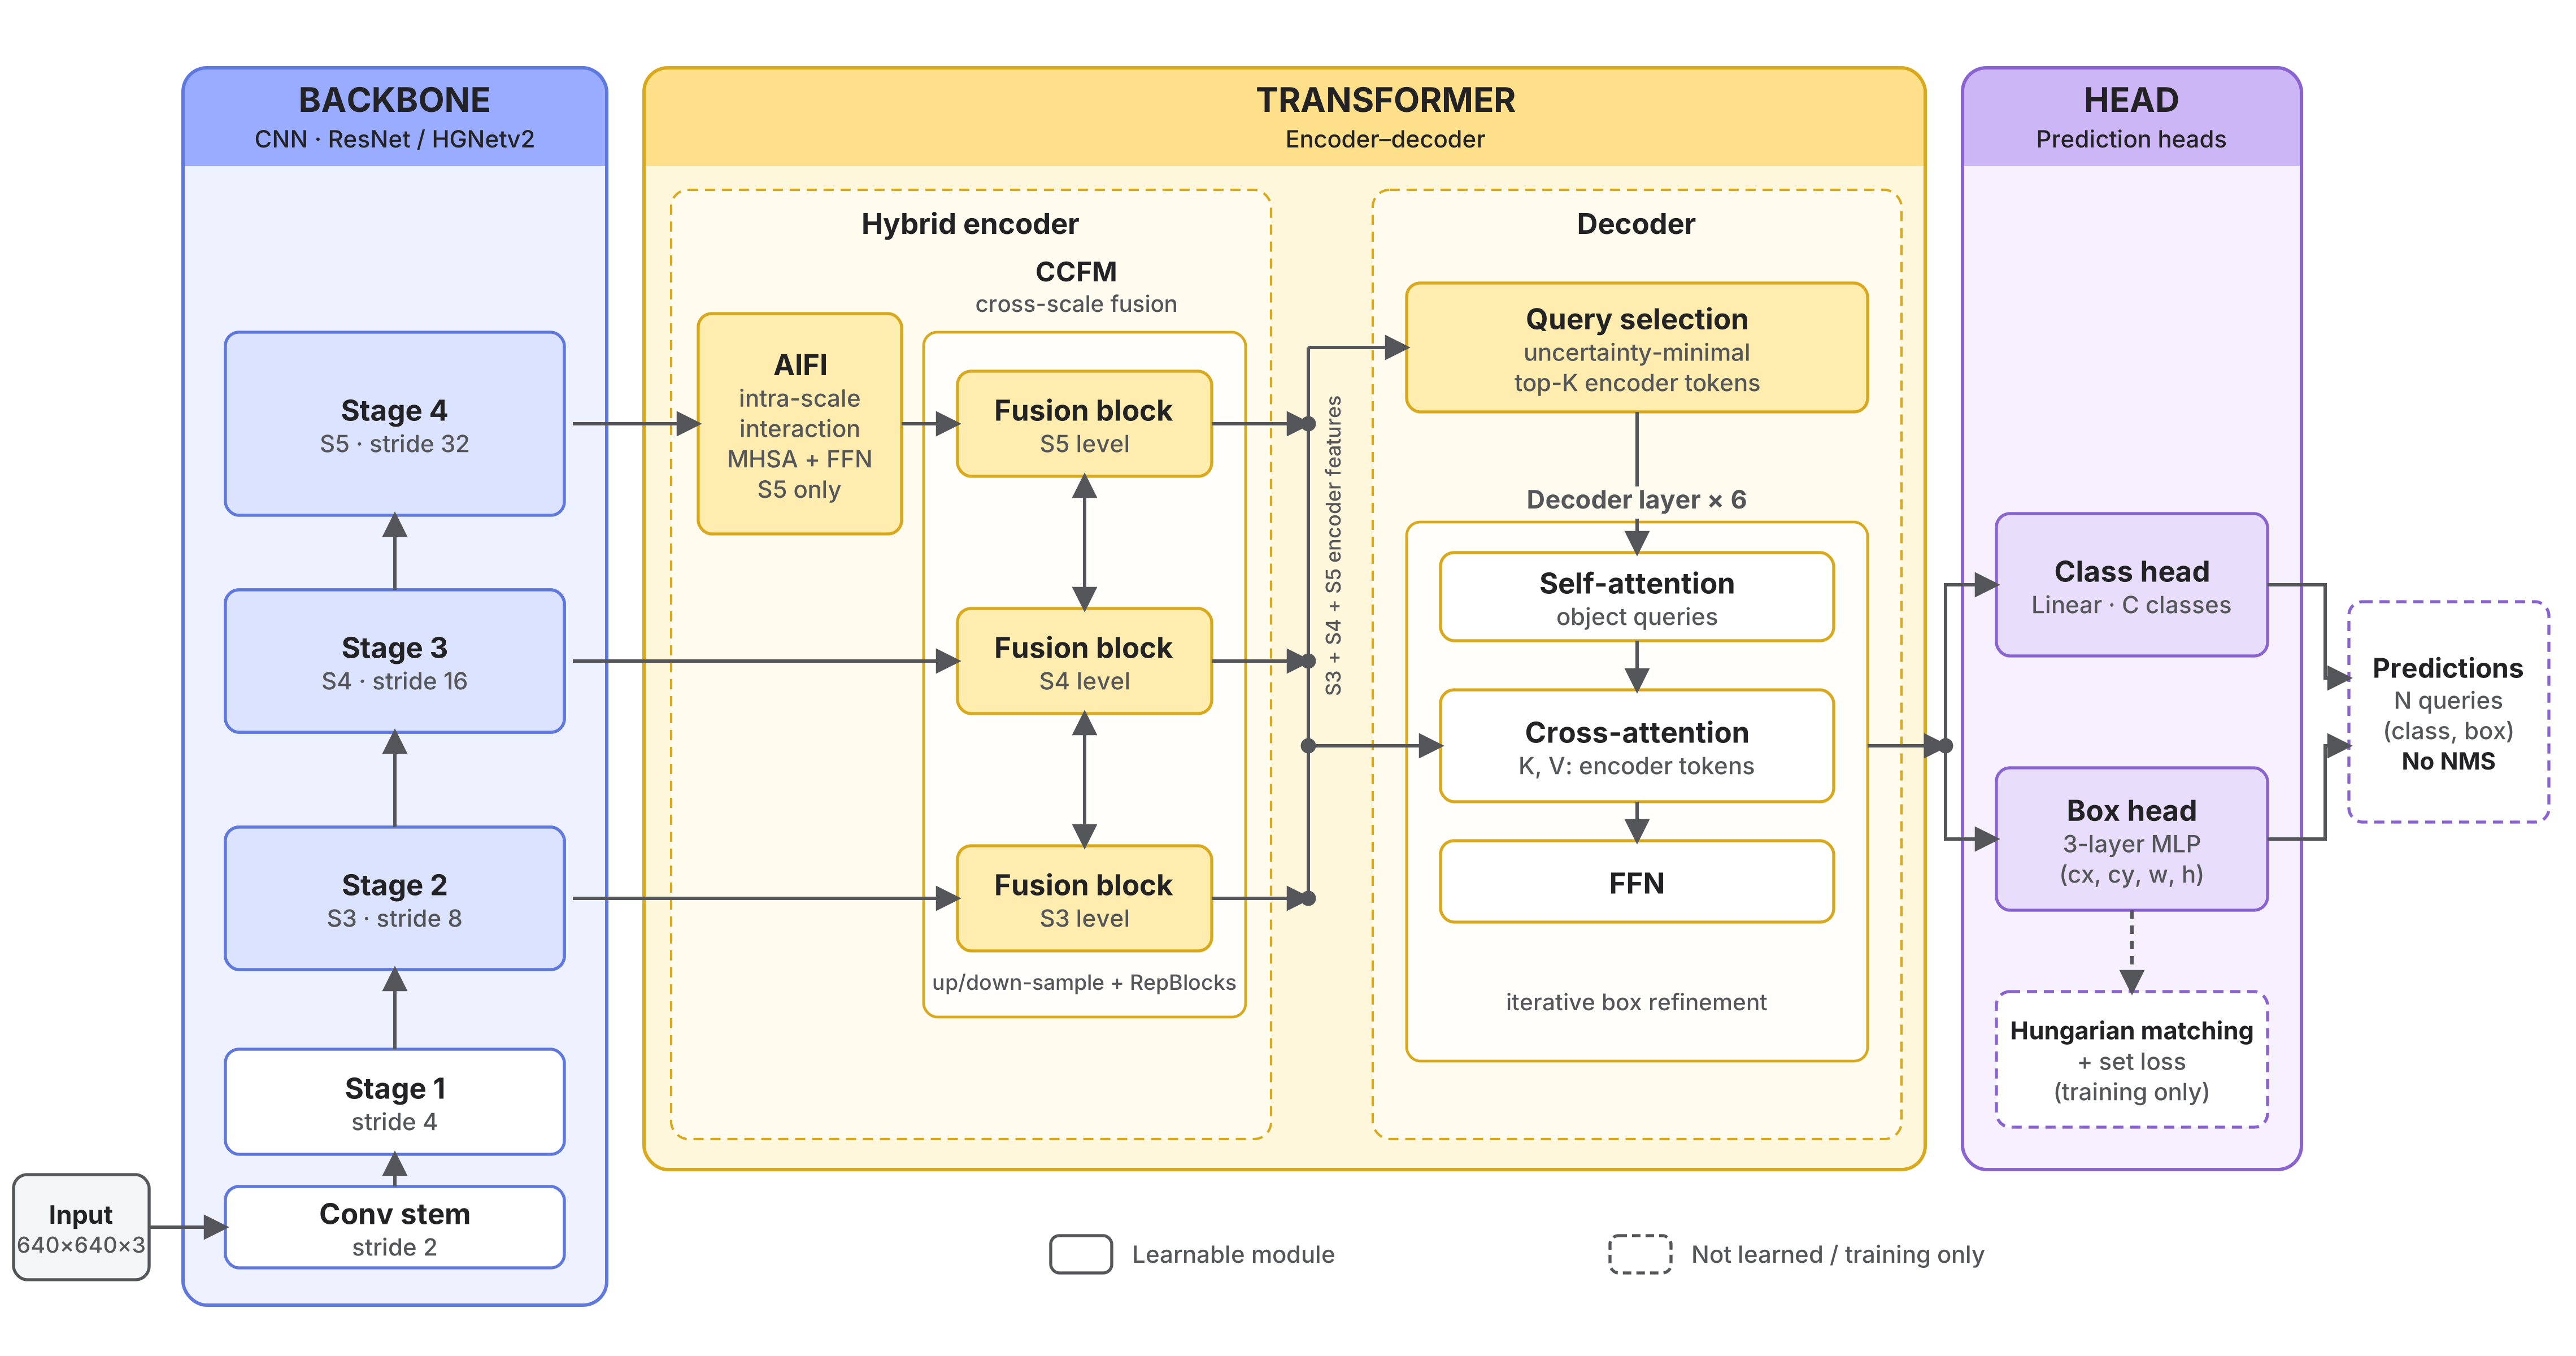
\includegraphics[width=\linewidth]{rtdetr_architecture (1).png}
\caption{RT‑DETR architecture: CNN backbone, hybrid encoder (self‑attention on high‑level features), cross‑scale feature fusion, decoder with query‑based set prediction, and separate class/box heads. No NMS is required at inference.}
\label{fig:rtdetr_arch}
\end{figure}

The DEtection TRansformer (DETR) represents a paradigm shift by treating object detection as a direct set prediction problem, removing the need for hand‑crafted components like anchor boxes and non‑maximum suppression. The architecture consists of a convolutional backbone, a transformer encoder‑decoder module, and specialized prediction heads. The backbone extracts low‑resolution feature maps from the input image, which are then flattened and combined with positional encodings. These features are processed by the transformer encoder‑decoder, which leverages self‑attention and cross‑attention mechanisms to model global context and object relationships before mapping them to a fixed set of object queries. Finally, the prediction heads, implemented as multi‑layer perceptrons, transform these queries into class labels and bounding box coordinates.
The DEtection TRansformer (DETR) represents a paradigm shift by treating object detection as a direct set prediction problem, removing the need for hand-crafted components like anchor boxes and non-maximum suppression. The architecture consists of a convolutional backbone, a transformer encoder-decoder module, and specialized prediction heads. The backbone extracts low-resolution feature maps from the input image, which are then flattened and combined with positional encodings. These features are processed by the transformer encoder-decoder, which leverages self-attention and cross-attention mechanisms to model global context and object relationships before mapping them to a fixed set of object queries. Finally, the prediction heads, implemented as multi-layer perceptrons, transform these queries into class labels and bounding box coordinates.

\section{Structured Pruning via L1-Norm}
\label{sec:pruning}
Structured pruning is a model compression technique based on the observation that deep neural networks are often overparameterized and contain redundant feature representations. The method aims to reduce model complexity by removing entire structural components, such as channels or filters, while preserving the overall architecture and predictive capability of the network. Unlike unstructured pruning, which removes individual weights and produces sparse parameter matrices, structured pruning removes complete computational units that can be directly accelerated on conventional hardware.

To identify which filters contribute minimally to the network's predictive performance, a common channel-importance criterion is derived from the L1-norm of the filter weights. The L1-norm provides a measure of the magnitude of the weights within a specific filter. For a given filter $W_i$ in a convolutional layer, the L1-norm is computed as
\begin{equation}
||W_i||_1 = \sum_{j} |w_{i,j}|,
\end{equation}

\begin{figure}[h]
\centering
\caption{Illustration of IoU taken from the Aedes egg dataset.}
\label{fig:iou_explainer}
\end{figure}
where $w_{i,j}$ represents the individual weight parameters within the $i$-th filter. Filters with a smaller L1-norm magnitude are considered to possess less structural importance and contribute less to the propagated feature representation. These filters are therefore selected as candidates for removal.

After ranking channels according to their importance scores, a pruning ratio $p$ is applied. If a layer initially contains $C$ output channels, the number of retained channels after pruning is given by
\begin{equation}
C_{\mathrm{retained}} = C(1-p).
\end{equation}

\begin{figure}[h]
\centering
\caption{Illustration of IoU taken from the Aedes egg dataset.}
\label{fig:iou_explainer}
\end{figure}

The removal of channels directly reduces both parameter count and computational complexity. For a convolutional layer with kernel size $K \times K$, $C_{\mathrm{in}}$ input channels, and $C_{\mathrm{out}}$ output channels, the total number of trainable parameters, excluding bias terms, can be expressed as
\begin{equation}
P = K^{2} \times C_{\mathrm{in}} \times C_{\mathrm{out}}.
\end{equation}

\begin{figure}[h]
\centering
\caption{Illustration of IoU taken from the Aedes egg dataset.}
\label{fig:iou_explainer}
\end{figure}

To illustrate the effect of structured pruning, consider a convolutional layer with $64$ input channels and $100$ output channels. Before pruning, the layer contains

\begin{equation}
P = 3^{2} \times 64 \times 100 = 57,\!600.
\end{equation}

\begin{figure}[h]
\centering
\caption{Illustration of IoU taken from the Aedes egg dataset.}
\label{fig:iou_explainer}
\end{figure}

Applying a pruning ratio of $20\%$ retains

\begin{equation}
C_{\mathrm{retained}} = 100(1-0.20)=80.
\end{equation}

\begin{figure}[h]
\centering
\caption{Illustration of IoU taken from the Aedes egg dataset.}
\label{fig:iou_explainer}
\end{figure}

The pruned layer therefore contains

\begin{equation}
P_{\mathrm{pruned}} = 3^{2} \times 64 \times 80 = 46,\!080,
\end{equation}

\begin{figure}[h]
\centering
\caption{Illustration of IoU taken from the Aedes egg dataset.}
\label{fig:iou_explainer}
\end{figure}

representing a $20\%$ reduction in the number of trainable parameters for the layer.

Consequently, reducing the number of output channels decreases the overall parameter count and the number of floating-point operations required during inference. This reduction enables more efficient deployment on resource-constrained edge devices while maintaining acceptable detection performance.

The theoretical foundation of structured pruning assumes that a neural network possesses sufficient representational redundancy such that low-importance channels may be removed without substantially affecting predictive accuracy. However, redundancy is not distributed uniformly throughout the network. In object detection models, the backbone, neck, and head components contribute differently to the overall framework. Since these modules serve distinct roles in feature extraction and prediction, the structural sensitivity to filter removal varies depending on whether pruning is directed at the convolutional backbone, the feature fusion networks, or the transformer-based prediction components.

\section{Knowledge Distillation}
\label{sec:kd}

Knowledge Distillation (KD) is a model compression technique in which a student model $\mathcal{S}$ learns under the supervision of a teacher model $\mathcal{T}$. In post-pruning fine-tuning, the original unpruned model serves as the teacher, while its structurally pruned counterpart serves as the student. The teacher provides additional supervisory information that can help the student preserve or recover predictive performance affected by structural pruning.

\subsection{Response-Based Distillation}

Response-based distillation transfers knowledge through the output predictions of the teacher. Given teacher and student logits $z_i^{\mathcal{T}}$ and $z_i^{\mathcal{S}}$, respectively, softened class probabilities are computed using a temperature parameter $T>0$:

\begin{equation}
p_i(z_i,T) =
\frac{\exp(z_i/T)}
{\sum_{j=1}^{C} \exp(z_j/T)}.
\end{equation}

\begin{figure}[h]
\centering
\caption{Illustration of IoU taken from the Aedes egg dataset.}
\label{fig:iou_explainer}
\end{figure}

where $C$ is the number of classes. Increasing $T$ produces a softer probability distribution, allowing relative probabilities between classes to convey additional information learned by the teacher.

The discrepancy between the teacher and student distributions is measured using the Kullback--Leibler (KL) divergence:

\begin{equation}
\mathcal{L}_{\mathrm{KD}}^{\mathrm{resp}} = T^2 D_{\mathrm{KL}}\left(p(\mathbf{z}^{\mathcal{T}}, T)\;||\;p(\mathbf{z}^{\mathcal{S}}, T)\right),
\end{equation}

\begin{figure}[h]
\centering
\caption{Illustration of IoU taken from the Aedes egg dataset.}
\label{fig:iou_explainer}
\end{figure}

where

\begin{equation}
D_{\mathrm{KL}}
\left(
p^{\mathcal{T}} || p^{\mathcal{S}}
\right)
\sum_{i=1}^{C}
p_i^{\mathcal{T}}
\log
\left(
\frac{p_i^{\mathcal{T}}}
{p_i^{\mathcal{S}}}
\right).
\end{equation}

\begin{figure}[h]
\centering
\caption{Illustration of IoU taken from the Aedes egg dataset.}
\label{fig:iou_explainer}
\end{figure}

The factor $T^2$ compensates for the reduced gradient magnitude introduced by temperature scaling. Minimizing this loss encourages the student to approximate the teacher's output distribution.

\subsection{Intermediate Feature-Based Distillation}

Feature-based distillation transfers knowledge through intermediate representations. This is particularly relevant to structured pruning, where removing channels modifies the internal feature representations of the student.

Let $F^{\mathcal{T}}$ and $F^{\mathcal{S}}$ denote corresponding feature maps from the teacher and student. When their dimensions differ, an adaptation function $\phi(\cdot)$ can align the student representation with the teacher:

\begin{equation}
\hat{F}^{\mathcal{S}} = \phi(F^{\mathcal{S}}).
\end{equation}

\begin{figure}[h]
\centering
\caption{Illustration of IoU taken from the Aedes egg dataset.}
\label{fig:iou_explainer}
\end{figure}

The feature alignment loss can then be formulated using mean squared error (MSE):

\begin{equation}
\mathcal{L}_{\mathrm{KD}}^{\mathrm{feat}}
\frac{1}{N}
\sum_{i=1}^{N}
\left(
F_i^{\mathcal{T}}
\hat{F}_i^{\mathcal{S}}
\right)^2,
\end{equation}

\begin{figure}[h]
\centering
\caption{Illustration of IoU taken from the Aedes egg dataset.}
\label{fig:iou_explainer}
\end{figure}

where $N$ represents the total number of feature elements. Minimizing this loss encourages the student to maintain intermediate representations similar to those of the teacher.

\section{Knowledge Distillation in Object Detection Architectures}
\label{sec:kd_architectures}

Applying knowledge distillation to object detection requires consideration of both intermediate features and detection outputs. Unlike classification, object detection involves predicting object classes and spatial locations across multiple feature scales. Therefore, knowledge can be transferred through feature representations, classification predictions, localization predictions, or combinations of these components.

\subsection{Distillation in YOLO Architectures}

In dense single-stage detectors such as YOLOv4 and YOLOv8, predictions are generated across multiple feature scales. Knowledge distillation can therefore be applied to both intermediate features and detection outputs. Feature-level distillation encourages the student to preserve useful representations, while prediction-level distillation encourages its outputs to approximate those of the teacher.

The overall distillation objective can be expressed as

\begin{equation}
\mathcal{L}_{\mathrm{total}}
\mathcal{L}*{\mathrm{task}}
+
\lambda*{\mathrm{resp}}
\mathcal{L}*{\mathrm{KD}}^{\mathrm{resp}}
+
\lambda*{\mathrm{feat}}
\mathcal{L}_{\mathrm{KD}}^{\mathrm{feat}},
\end{equation}

\begin{figure}[h]
\centering
\caption{Illustration of IoU taken from the Aedes egg dataset.}
\label{fig:iou_explainer}
\end{figure}

where $\mathcal{L}*{\mathrm{task}}$ denotes the object detection loss, while $\lambda*{\mathrm{resp}}$ and $\lambda_{\mathrm{feat}}$ control the contributions of response- and feature-based distillation.

\subsection{Distillation in RT-DETR}

For transformer-based detectors such as RT-DETR, knowledge distillation must account for the set-based nature of object predictions. Since object queries do not necessarily have a fixed correspondence between teacher and student predictions, distillation can be performed through prediction alignment and intermediate feature representations.

At the prediction level, an assignment between teacher and student queries can be established using a matching function:

\begin{equation}
\hat{\sigma}
\arg\min_{\sigma \in \mathfrak{S}*{N_q}}
\sum*{i=1}^{N_q}
\mathcal{L}_{\mathrm{match}}
\left(
\hat{y}*i^{\mathcal{T}},
\hat{y}*{\sigma(i)}^{\mathcal{S}}
\right),
\end{equation}

\begin{figure}[h]
\centering
\caption{Illustration of IoU taken from the Aedes egg dataset.}
\label{fig:iou_explainer}
\end{figure}

where $N_q$ is the number of object queries and $\mathfrak{S}_{N_q}$ represents the set of possible query permutations. Once corresponding predictions are established, classification and localization information can be transferred between the teacher and student.

Feature-level distillation can similarly be applied to the intermediate representations of the transformer encoder:

\begin{equation}
\mathcal{L}_{\mathrm{enc}}^{\mathrm{DETR}}
\frac{1}{N_kD}
\sum_{k=1}^{N_k}
\left|
H_k^{\mathcal{T}}
\psi(H_k^{\mathcal{S}})
\right|_2^2,
\end{equation}

\begin{figure}[h]
\centering
\caption{Illustration of IoU taken from the Aedes egg dataset.}
\label{fig:iou_explainer}
\end{figure}

where $N_k$ is the number of feature tokens, $D$ is the embedding dimension, and $\psi(\cdot)$ is a projection function used to align the student representation with the teacher.

\section{Network Quantization}
\label{sec:quantization}

Network quantization is a model compression technique that reduces the numerical precision of weights and activation maps from 32-bit floating-point ($\text{FP32}$) to lower-bit representations, typically 8-bit integers ($\text{INT8}$) \cite{Jacob2018, Krishnamoorthi2018}. Converting parameters to $\text{INT8}$ reduces physical storage requirements by approximately 75\% and enables integer-arithmetic acceleration on target edge hardware \cite{Nagel2021}.

\subsection{Uniform Linear Quantization}

The continuous real-valued tensor $x \in [x_{\min}, x_{\max}]$ is mapped to a discrete integer $q \in [q_{\min}, q_{\max}]$ through uniform linear quantization:
\begin{equation}
q = \text{clip}\left( \left\lfloor \frac{x}{S} \right\rceil + Z, \; q_{\min}, \; q_{\max} \right),
\end{equation}

\begin{figure}[h]
\centering
\caption{Illustration of IoU taken from the Aedes egg dataset.}
\label{fig:iou_explainer}
\end{figure}
where $S \in \mathbb{R}^{+}$ is the positive scale factor, $Z \in \mathbb{Z}$ is the integer zero-point offset, and $\lfloor \cdot \rceil$ represents rounding to the nearest integer. For signed $\text{INT8}$, the discrete bounds are $[q_{\min}, q_{\max}] = [-128, 127]$ \cite{Krishnamoorthi2018}. 

During inference, approximate floating-point values $\hat{x}$ are recovered via dequantization:
\begin{equation}
\hat{x} = S \cdot (q - Z).
\end{equation}

\begin{figure}[h]
\centering
\caption{Illustration of IoU taken from the Aedes egg dataset.}
\label{fig:iou_explainer}
\end{figure}

\subsection{Symmetric versus Asymmetric Schemes}

Quantization schemes are categorized by how real zero is mapped into the discrete integer range \cite{Nagel2021}:
\begin{itemize}
    \item \textbf{Asymmetric Quantization:} Maps $[x_{\min}, x_{\max}]$ across the full integer range using a non-zero zero-point ($Z \neq 0$). This scheme preserves precision for skewed or strictly non-negative activation distributions (e.g., post-$\text{ReLU}$ or $\text{SiLU}$ feature maps).
    \item \textbf{Symmetric Quantization:} Enforces $Z = 0$ by aligning real zero with integer zero. The dequantization simplifies to $\hat{x} = S \cdot q$, eliminating zero-point subtraction logic during matrix multiplication and optimizing hardware execution.
\end{itemize}

\subsection{Quantization Granularity and Post-Training Calibration}

Quantization can be applied at different structural levels \cite{Nagel2021}:
\begin{itemize}
    \item \textbf{Per-Tensor vs. Per-Channel:} Per-tensor quantization shares a single scale factor $S$ across an entire layer, whereas per-channel quantization assigns an independent scale $S_c$ to each output channel $c$. Per-channel scaling is typically applied to convolutional weights to prevent large-magnitude filters from dominating subtle feature channels.
    \item \textbf{Post-Training Quantization (PTQ) Calibration:} PTQ quantizes the network without full retraining \cite{Nagel2021}. While weight distributions are fixed, dynamic activation ranges are determined by passing a small calibration dataset through the unquantized model to establish optimal scale factors $S$ (e.g., via MinMax or KL-divergence range estimation).
\end{itemize}

\subsection{Quantization Dynamics in Object Detectors}

Applying integer quantization to object detection architectures involves component-specific considerations:
\begin{itemize}
    \item \textbf{YOLO Feature Fusion Layers:} Concatenation nodes in the feature pyramid neck merge shallow, high-magnitude features with deep, localized semantic features. Joint calibration ensures scaling factors do not truncate small-activation responses crucial for small-object localization.
    \item \textbf{Transformer Attention Blocks:} Linear projection layers in RT-DETR map cleanly to $\text{INT8}$, but non-linear Softmax operations within multi-head self-attention remain sensitive to precision loss. Softmax and normalization layers are retained in floating-point precision ($\text{FP32}$) to preserve attention score stability \cite{Nagel2021}.
\end{itemize}
\section{Evaluation Metrics}
To rigorously assess the performance of the object detection models before and after compression, standard quantitative metrics are utilized. The foundational metric for spatial localization is Intersection over Union (IoU), which measures the overlap between the predicted bounding box $\mathcal{B}_p$ and the ground truth bounding box $\mathcal{B}_{gt}$:

\begin{figure}[h]
\centering
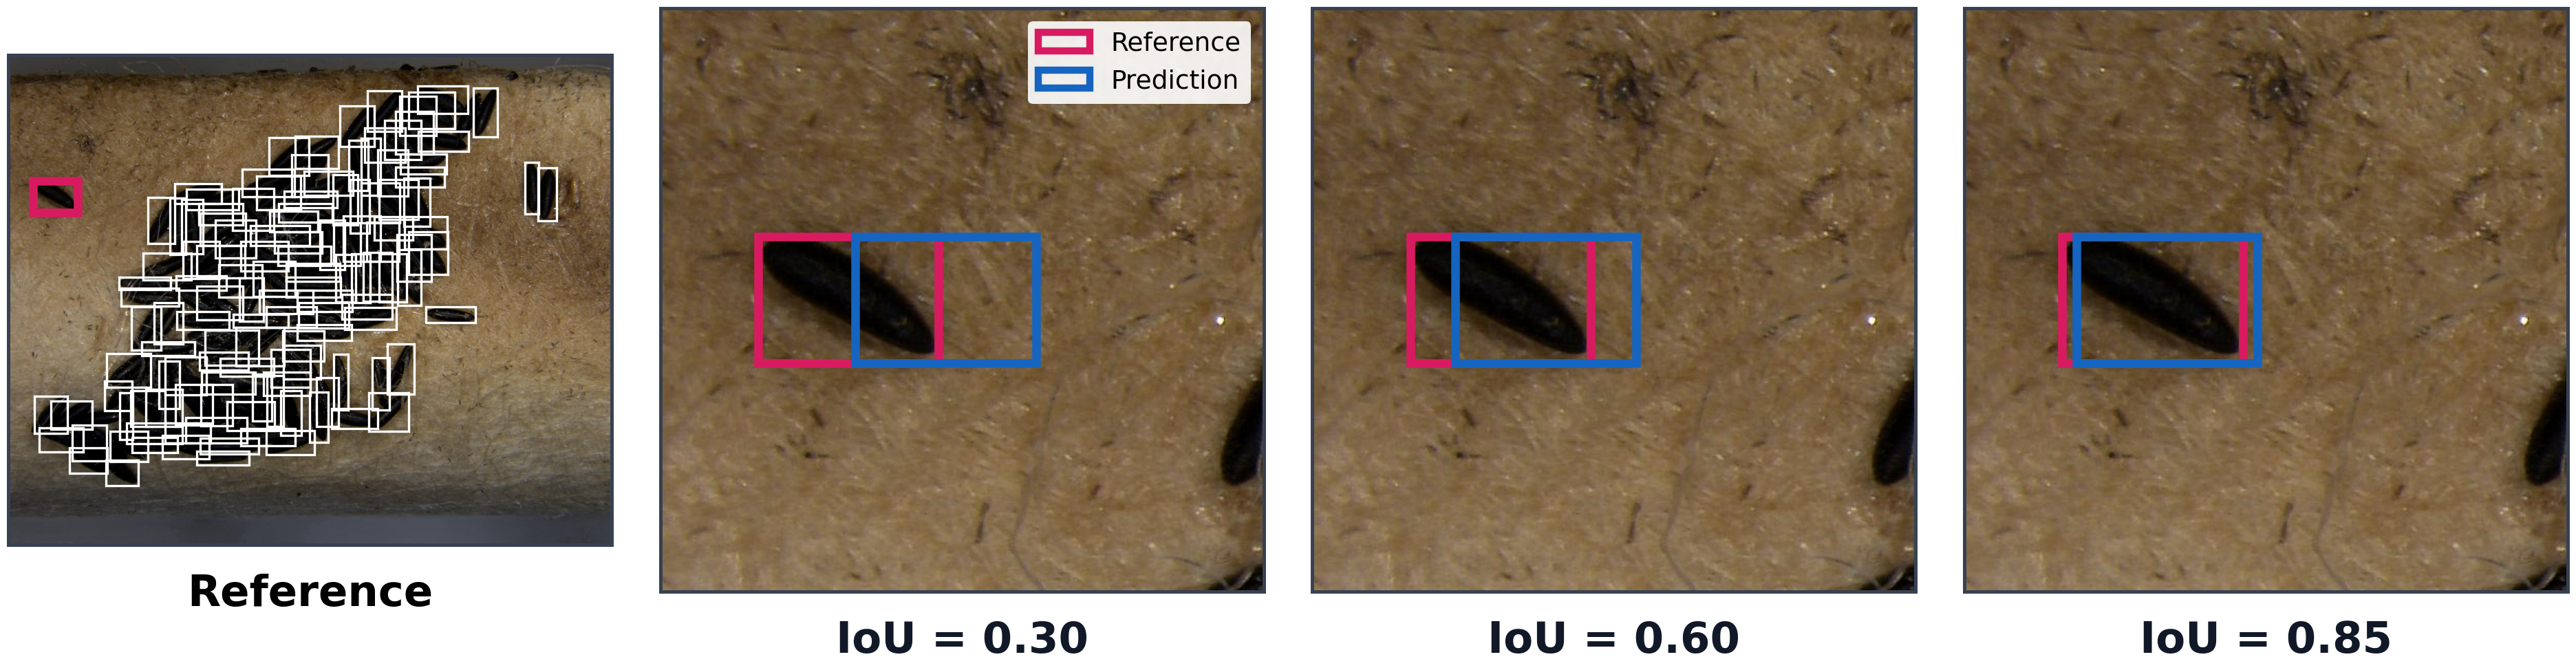
\includegraphics[width=\linewidth]{main_mosquito_iou_explainer.png}
\caption{Illustration of IoU taken from the Aedes egg dataset.}
\label{fig:iou_explainer}
\end{figure}
\begin{equation}
\mathrm{IoU} = \frac{\mathrm{Area}(\mathcal{B}_p \cap \mathcal{B}_{gt})}{\mathrm{Area}(\mathcal{B}_p \cup \mathcal{B}_{gt})}.
\end{equation}

\begin{figure}[h]
\centering
\caption{Illustration of IoU taken from the Aedes egg dataset.}
\label{fig:iou_explainer}
\end{figure}

A prediction is classified as a True Positive (TP) if the IoU exceeds a predefined threshold and the class prediction is correct. Otherwise, it is classified as a False Positive (FP). Ground truth objects that the model fails to detect are False Negatives (FN). These values are used to calculate Precision and Recall:
\begin{equation}
\mathrm{Precision} = \frac{\mathrm{TP}}{\mathrm{TP} + \mathrm{FP}},
\end{equation}

\begin{figure}[h]
\centering
\caption{Illustration of IoU taken from the Aedes egg dataset.}
\label{fig:iou_explainer}
\end{figure}
\begin{equation}
\mathrm{Recall} = \frac{\mathrm{TP}}{\mathrm{TP} + \mathrm{FN}}.
\end{equation}

\begin{figure}[h]
\centering
\caption{Illustration of IoU taken from the Aedes egg dataset.}
\label{fig:iou_explainer}
\end{figure}

Precision quantifies the accuracy of the positive predictions, while Recall quantifies the model's ability to identify all relevant instances. The overall detection capability is summarized using Average Precision (AP), which is calculated as the area under the Precision-Recall curve $p(r)$:
\begin{equation}
\mathrm{AP} = \int_{0}^{1} p(r) \, dr.
\end{equation}

\begin{figure}[h]
\centering
\caption{Illustration of IoU taken from the Aedes egg dataset.}
\label{fig:iou_explainer}
\end{figure}

Mean Average Precision (mAP) is subsequently derived by calculating the mean of the AP values across all defined object classes, providing a comprehensive single-value metric for overall model reliability.





\begin{itemize}

\item \url{https://link.springer.com/chapter/10.1007/978-1-4419-1454-5_12}
\item \url{https://link.springer.com/article/10.1007/s10972-015-9443-2}



\end{itemize}



